% Chapter 2 - Background

% \glsresetall % reset the glossary to expand acronyms again
\chapter[Background]{Background}\label{ch:Background}
\index{Background}

If you really want to blame someone for the existence of this thesis, I would hang it on John Gufstason for proposing weak scaling \cite{Gustafson1988GustafsonLaw}.
Gustafson's Law states that if you can solve a parallelized problem on a computer in a fixed amount of time, you should be able to scale the problem size and the parallelized compute to solve a larger problem in the same amount of time.
In other words, the larger the computer, the larger the problems it can solve.
This foundational idea makes up the bedrock of \textit{high-performance computing} (HPC), and many decades of research have been poured into building larger and more parallel systems to solve bigger and more challenging problems.

The world's most powerful computers have been growing at an exponential pace for the past decade, with each generation providing more parallelism and being able to solve larger problems \cite{Top500}.
Recently the world's most powerful supercomputer, Frontier \cite{Frontier}, broke the exascale barrier with the ability to calculate $1.68*10^{18}$ 64-bit floating point operations per second (FLOPS). 
While breaking the exascale barrier is a monumental achievement, with over a decade of planning and research funded through the \textit{exascale compute project} (ECP), large numbers like $10^{18}$ are hard to understand without context.
ExaWind \cite{ExaWind} is an ECP project with the goal of developing large-scale simulations of wind farms, scientists and engineers have always been able to use \textit{computational fluid dynamics} (CFD) to evaluate their designs, but the deployment of larger computers is crucial to unlocking larger and higher fidelity simulations.
For example, in the mid-2000s, high-end systems would only have the capability to simulate a single blade, systems deployed in the 2010s let researchers scale their simulations to a full turbine with three blades rotating, creating turbulence.
Exascale is projected to enable simulations at wind-farm scale so that designers can account for turbine-to-turbine turbulence, the impact of terrain, be it land or off the coast, and atmospheric conditions like weather patterns.
But CFD isn't the only field extreme scale systems can enable new capabilities, many other fields rely on HPC, including molecular dynamics, cosmology, quantum chemistry, drug discovery and even \textit{artificial intelligence} (AI)/\textit{deep learning} (DL). 

The consequence of relentless innovation in HPC systems is that current systems are incredibly complicated.
To achieve massive scale within a reasonable power budget, modern HPC systems consist of a high-performance fabric connecting compute nodes densely packed with GPUs and multi-core CPUs.
This leads to complex memory hierarchies with technologies like \textit{non-uniform memory access} (NUMA), CPU caches, and GPU memory; all of which are tied together with high-performance interconnects like \textit{Peripheral Component Interconnect Express} (PCIe), Intel's \textit{Ultra Path Interconnect} (UPI), NVLink, and InfiniBand.
Now, to squeeze the most performance out of these expensive machines, domain scientists need to account for all of this complexity and map it to whatever insanely difficult grand challenge they are trying to solve.
In other words, writing efficient code for these massive systems is very hard.

This is where scientific programming libraries like come in.
Over the years, academics and industry have congealed on a set of standards and abstractions for the hardware so that it can be more easily manipulated at a higher level.
While programming multi-core CPUs is possible with pthreads \cite{pthreads}, it is often easier for scientists to use OpenMP \cite{OpenMP} because it provides a friendlier interface that is easier to map to scientific problems.
Many applications built on GPUs use Nvidia's \textit{Compute Unified Device Architecture} (CUDA) \cite{CUDA} to drive the GPU, but scientists are slowly pushing for open-source alternatives like Kokkos \cite{kokkos}, Raja \cite{Raja}, and even OpenMP so that they're not locked into a single vendor's programming library.
Driving the network can be done using shared-memoryesque libraries based on \textit{Partitioned Global Address Space} (PGAS), with popular models including SHMEM \cite{OpenSHMEM}, \textit{Unified Parallel C} (UCP) \cite{UPC}, and Chapel \cite{Chapel}; but the point-to-point based \textit{Message Passing Interface} (MPI) \cite{mpi40} is by far the most prevalent programming model for managing distributed memory systems.
MPI's dominance can be attributed to its well-established and respected standardizing body, but mostly because it's easy to understand and provides a powerful yet simple programming model for domain scientists to scale their problems to the largest machines. 

MPI is a critical piece of HPC infrastructure, since its inception in the early 90s, developers have been adopting it as the distributed memory library of choice.
Being such a fundamental piece of scientific computing leads to many codes relying on the MPI's implementation to be as performant as possible.  
It is not uncommon for application performance to be bound by the time spent in MPI, with many applications able to spend over 50\% of their time processing MPI calls \cite{Chunduri2018CharacterizeMPIonProd}.
Collective communications, an MPI primitive that organizes simultaneous data exchanges among groups of processes, tend to consume large amounts of core hours and can become a bottleneck of many large-scale applications.
A specific example includes \textit{Deep Learning} (DL), these frameworks heavily rely on MPI\_Allreduce to implement model parallelism, and applications like Horovod frequently issue large message Allreduce on GPU buffers to exchange weight updates \cite{Awan2019CommProfDLonClusters, Jain2019PerfCharDNNTFPT, Alizadeh2022PAPCollDL}.
Therefore, it is paramount that MPI latency is as minimal as possible because time spent in MPI is time wasted not calculating science, and often the pace of computational sciences is bound by the speed of MPI.

The rest of this chapter will establish the fundamentals of HPC from the bottom up.
It starts with a deep dive into the node architecture, discussing the trend of heterogeneous clusters, then scaling up to the system level to evaluate the technologies interconnecting all the compute islands.
Next, the software environment is established, since this thesis is focused on communication libraries, we start with 'transport-layer' libraries which are used to build MPI implementations, then we discuss MPI itself, why it's prevalent, and its important features. % then we provide an example of an application that makes heavy use of MPI, driving the motivation to research certain aspects of MPI itself.

\section{GPU Cluster Architecture}
Modern HPC is performed on GPU clusters, which are, in essence, a bunch of nodes (rack-mounted servers) tied to a system area network.
These machines are assembled using commodity parts, and system designers can integrate components from different vendors.
The fundamental components include the CPU, GPUs, and the interconnect, all of which have different vendors providing different solutions with their own price/performance/density tradeoffs.
This allows for all kinds of flexible deployments, with the most obvious benefit being cost, but designs can be tailored to based on application (weather modelling, nuclear simulations, deep learning) or based on component supply (if there's ever some global disruption to supply chains or whatever and your lab can't get ahold of the network cards you wanted).
While designers have flexibility in their deployments, several concepts and technologies  are consistent across deployments.

The components in a cluster can be grouped into two categories, they either perform compute, or they are moving data between compute endpoints.
Within a compute node, both CPUs and GPUs can perform compute, and there are a series of interconnects like PCIe and NVLink that shuffle data between compute resources.
And at a larger scale, each node can be considered a compute island while the network shuffles data between nodes.
Each resource has its quirks, and applications need to be properly structured to make full use of system resources, and at the same time, it is the library designer's job to provide tools that efficiently expose the granularity of control that developers need without overwhelming them with hardware details.

There is an additional category of components focused on accelerating file I/O.
These components can include node-local SSD or Intel's Optane persistent memory, and they are used to expose a higher-performance file system with better bandwidth and latency than traditional network-attached storage.
While these tools are important, and many applications are file I/O bound, these tools are out of the scope of this thesis. 

\subsection{Compute Node Architecture}
The compute nodes are where the calculations happen.
The design goal of a compute node is to be able to perform as many FLOPS as possible while minimizing power consumption and area.
At a high level, a node can be thought of as a rack in a server tying together memory, CPUs, GPUs, network cards, and maybe a bit of local storage, but there is nuance to node design and tradeoffs that determine component selection. 

\subsubsection{CPU Compute Nodes}
Traditionally, compute nodes would be entirely CPU based, powered by multiple sockets of SMP cores.
Typical CPU nodes can have in the range of 32 to 128 cores per node depending on the CPU model, and each CPU has their own memory controllers attached to a pool of memory ranging from 128GB to 4TB.
Thanks to the operating system technology, multiple CPU sockets are combined and presented to applications as a single giant CPU attached to a giant pool of memory, and processes running on any core can access memory from any memory bank attached to any other CPU.

Now, this model is known as a \textit{Symmetric Multiprocessor} (SMP), where processes share a common memory bus, and any thread can access any other process' memory, but in reality, these systems are not exactly symmetric. 
Since each socket has its own memory controllers, each socket has its own NUMA domain, and there is a performance penalty accrued when cores access memory in other process's memory domains.
There are also complex cache hierarchies, and if two cores are frequently modifying the same memory location, the contention caused by frequent cache flushes will tank performance, this is also known as cache thrashing.
So when writing parallelized code, application developers must consider where data resided in memory and how CPU cores access that data.
 
The number of cores in CPU-based SMP architectures has been growing slowly over the past decade, with high-end systems topping out around 128 cores (256 if you consider hyperthreading).
The trouble with CPU cores is that they're complicated, the x86 instruction set has been around since the 80s and has been expanded multiple times, there are \textit{single instruction multiple data} (SIMD) for vectorization, security extensions for the paranoid, and even compatibility modes for older 32-bit programs. 
There are alternate RISC ISA that cut down on instruction complexity, with the most mature being ARM, but these cores are still heavily optimized for single-thread compute.
Compared to other core architectures, CPU cores tend to be large and not very space efficient. 

\subsubsection{GPU Compute Nodes}
GPUs subvert the core-complexity problem of CPUs by greatly simplifying the core design and providing thousands of cores per chip. 
These accelerators provide massively parallel banks of floating point compute, and they can spit out so many FLOPS they require specially manufactured high bandwidth memory (HBM) to feed the beast.
In terms of FLOPS/mm$^2$ and FLOPS/Watt, GPUs win out by orders of magnitude, which is one of the largest driving reasons why GPU adoption for compute-intensive applications has exploded over the past decade.
You can also associate multiple GPUs to a single CPU, so the trend has been to pack as many GPUs into a node as possible.
When GPUs first took first place on the Top500 with Titan at ORNL, there was a single GPU per node, but a decade later, Frontier has scaled up to eight GPUs per node (technically, there are four MI250x cards per node, but each card has two GPU dies tied together with some advanced packaging solution, and it's presented to the application as eight GPUs).

But, these external accelerators also add considerable amounts of complexity to system design, and that complexity is felt most acutely at the software level.  
Because GPUs are fundamentally different from CPUs, they require special programming models.
Programmers specify GPU-bound parallel computations in a GPU kernel, and at run-time, kernels are launched in parallel across a user-specified number of threads.
To save die space, GPU cores discard bloat like branch predictors, so control flow inside compute kernels can destroy performance if not accounted for properly.
Since thousands of threads can run simultaneously, even more attention has to be paid to memory access patterns, as there is even more potential  for sloppy code to tank performance (see memory coalescing \cite{CUDAMemCoalescing}).
There's also the fact that GPUs have their own HBM that can't be accessed by load/store CPU instructions, and GPU kernels can only access data resident to the card they're running on, so device data management is another challenge developers need to account for. 
But when everything comes together, when memory accesses are coalesced, when there is no warp divergence, when CPU-GPU memory transfers are overlapped with compute, and all required sweat/blood sacrifices have been performed, holy cow are GPUs fast.

\subsubsection{Interconnects}
Within a node, data can reside in host memory or device memory, host memory can be further subdivided into NUMA domains, and there are often multiple GPUs with their own memory domains.
So data is constantly being shuffled between different types of memory, and to accommodate this, the hardware interconnecting different memory regions needs to be as fast as possible.
Several technologies have been designed to support these operations, with broad categories including cross-socket CPU-CPU interconnects, host-to-device interconnects, and  GPU-GPU  interconnects.

For multi-socket shared memory systems to work properly, there needs to be a hardware mechanism to maintain memory and cache coherency between the CPUs.  
The technology behind these solutions is often proprietary and vendor-specific, with each CPU vendor having their own implementation.
For example, Intel's Xeon Scalable processors can be connected through UPI \cite{XeonTechOverview}.
Xeon CPUs have either two or three UPI links (depending on SKU), which can transfer data at 10.4GT/s and can be combined into different topologies of two, four, or eight CPUs.
Intersocket link designs are often tightly coupled to the on-chip memory controllers, seeing as their job involves connecting said memory controllers across sockets.
These interfaces strive to be transparent to applications, so programming for these interfaces is not that explicit and often involves critically thinking about thread/process-to-core bindings and ensuring compute kernels aren't cache thrashing.

To move data in and out of accelerator memory, systems leverage \textit{Peripheral Component Interconnect Express} (PCIe).
The PCIe standard, maintained by the PCI-SIG consortium, was first released in 2003 and has evolved over the years to meet ever-increasing communication needs \cite{PCIeIntroPaper, PCIeV5Spec}.
A PCIe connection is based on a scalable number of lanes, which represent the physical wires connecting the endpoints, and can range from a single lane up to 16 lanes, with more lanes providing more bandwidth.
At the time of writing, the most common implementation is PCIe V4 which provides bidirectional 2GB/s per lane, letting high-performance devices top out at 32GB/s on a 16x connection. 
PCIe is also a switched architecture, for example, it is possible to design a system where a 16x CPU endpoint coming off the CPU can be passed into a switch and connected to four GPUs with their own 16x endpoints.
The PCIe standard isn't just for accelerators, it is designed to work for any I/O device and is also used to connect storage devices and network cards to the CPU.
Many operations traverse PCIe transparently, for example, all network operations traverse PCIe, and all file I/O operations pass a PCIe connection, both local and network attached.
In most GPU programming models, the host-to-device transfers are explicit through functions like cudaMemcpyAsync, so developers will know when transfers are taking place and can use techniques like compute-communication overlap to hide transfers.

The last category of connections is GPU to GPU interconnects, and there are several technologies here, both proprietary and open.
Originally, if a system had multiple GPUs, transfers would have to be staged through host memory, but it is possible for GPUs to send data to each other through PCIe peer-to-peer.
This technology cuts host memory out of the data's path, increasing bandwidth and freeing up CPU resources to handle other tasks.
But the pace of development for PCIe is relatively slow since consortiums are not fast in publishing new standards. 
Since PCI-SIG can't keep up with the scaling bandwidth requirement of HPC, GPU manufacturers have started to create their own device-to-device connections.
For example, Nvidia's GPUs can leverage NVLink.
NVLink3, the third generation of NVLink announced alongside the A100 GPU, can transmit data at 50Gb/s per lane and has an accompanying NVSwitch for scalability \cite{A100Whitepaper}.
Each A100 GPU has 12 links, providing system designers with the flexibility to build different topologies, for example, four GPU nodes can have a fully-connected topology with each GPU connected by a 200Gb/s pipe, or an ultra-dense eight GPU node can leverage six NVSwitches in parallel to build a star topology.
These connections can be orders of magnitude faster than PCIe and are tightly integrated with the GPUs memory controller.
Programmatically, developers drive NVLlink through cudaIPC, a model similar to mapped memory where a memory handle from one GPU is passed to another GPU through main memory, then compute kernels can access the remote memory region as if it is local memory.

\subsection{The Network}
The last and most critical piece of a cluster is the network.  
A single node will have some inherent scalability limit often bottlenecked by compute (number of CPU cores or GPUs) or memory (the number of memory channels the CPU can support or the available GPU memory).
HPC Clusters break this limit by tying multiple nodes together through a high-bandwidth and low-latency network so that programmers can scale their application across the resources of multiple nodes.
But once again, adding this extra layer for scalability adds a bunch more complexity that needs to be accounted for.

\begin{figure}[h]
	\centering
	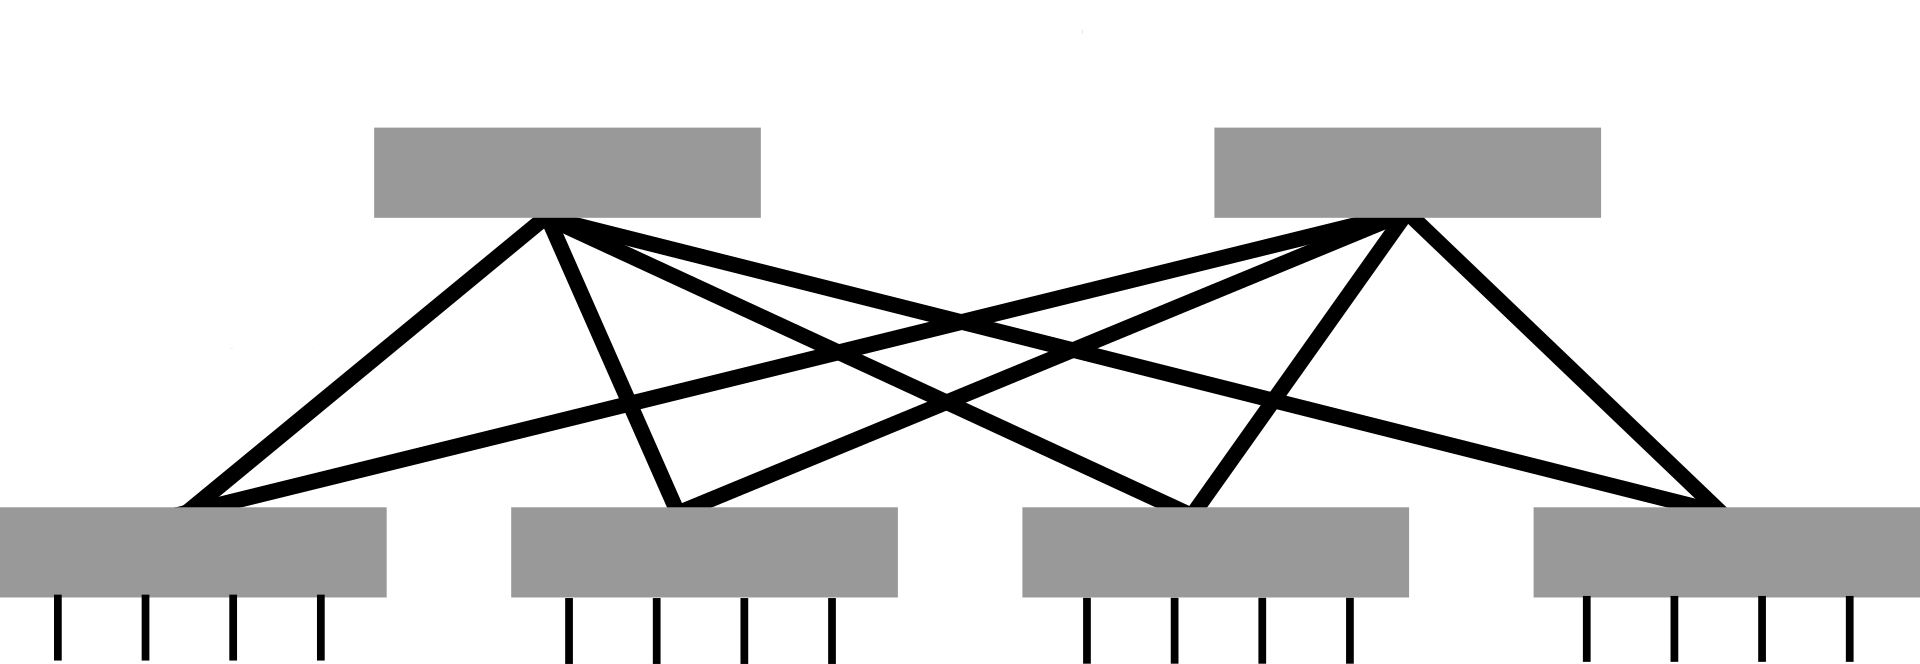
\includegraphics[width = 4.5in]{3_Chapters/2_Chapter_Background/Figs/FatTree.png}
	\caption[Sample fat tree network]{
     Sample fat tree network.
     There are 16 nodes, connected to 4 leaf switches, connected to 2 spine switches acting as the root.
     The thickness of each link represents its bandwidth.
     }
	\label{fig:fat-tree-topology}
\end{figure}


The network topology describes how the nodes are connected, it is often modelled as a graph where vertices are either nodes or switches, and edges represent the network links connecting resources.
In the past, large systems would deploy switchless fabrics, with popular topologies including mesh and torus networks.
Some production clusters still use switchless networks as they map well to the communication patterns of certain HPC applications, but modern commodity hardware has converged on switched topologies, as they are easier to deploy, scale, and manage. 
There are many switched topologies used in practice and proposed in the literature, popular ones include Clos and dragonfly, but the most common switched topology deployed in HPC clusters is fat-tree.
A sample fat tree topology with 16 nodes and two levels is demonstrated in Figure \ref{fig:fat-tree-topology}, similar to a tree data structure, there is a spine switch (the root of the tree) connected to leaf switches (children of the root) which connect to the nodes (leaves of the tree).
Fat-tree get their name because links at the top of the tree will have more bandwidth than links at the bottom, this is because all nodes can potentially send data across the root at the same time.
To save costs, fat trees can be designed with a blocking factor which describes the ratio of available bandwidth at the root compared to the number of children attached to a leaf node, so a non-blocking fat-tree can afford to have all nodes send data across the root at the same time, while a tree with a 5:1 blocking ratio will grind down to 1/5 of the potential bandwidth if all processes go through the spine at the same time.

In HPC communities, the most widely adopted type of network is InfiniBand. 
Similar to PCIe, InfiniBand is a networking standard published by the \textit{InfiniBand Trade Association} (IBTA).
The first InfiniBand spec was published in 2001 with hardware that could support speeds around two Gb/s, but over time the standard and technology have evolved, and now modern InfiniBand networks can transfer data at 400 Gb/s.
The other key characteristic of an HPC network is tremendously low latency, network designers have poured countless hours into removing any possible overhead from the communication code path, some of these key technologies include kernel bypass, hardware tag matching, and network offload.
The InfiniBand specification outlines both the physical characteristics of the network hardware, as well as the InfiniBand verbs programming interface \cite{IBSpec}.
InfiniBand is not the only programming interface, though, and many players have moved in and out of the HPC networking market.
Cornelis Networks develops OmniPath, and Cray has their own line of SlingShot networks, all of which share similar performance and foundational ideas in their design but differ enough to fall across a diverse price/performance spectrum.

\section{Communication libraries} 

There are limits to how applications can interact with the network.
Modern networks have message latencies on the order of microseconds, but with L1 cache latency being on the order of nanoseconds, network transfers are excruciatingly slow.
With drastic performance limits that need to be designed around and a diverse set of network hardware to choose from, a unique set of programming tools are needed to expose network resources. 
There are vast differences in vendor technology as well, different networks have different software layers built on top of them, and portability between networks is an important requirement for many applications. 
So over time, a series of APIs have formed, each targeting different types of users, exposing more/less granularity of the hardware and different types of convenience functions designed to help write code for each layer.
The lowest layer would be device-specific libraries, these are vendor-specific data structures and functions designed to interact directly with hardware on the network card.
Above the device layer would be the transport layer, these are APIs that are designed to lightly wrap around different communication endpoints, they are still not that user-friendly, but they provide more portability and can more easily manage different sets of resources.
The transport layer is used to build programming models, the best example of which is MPI, this is the layer application developers are expected to interact with, it provides the most flexibility and portability for scientific codes.

\subsection{Device APIs and the Transport Layer}

The lowest possible layer of network software are device-specific interfaces, and each vendor has their own; for example, InfiniBand has verbs, Cray's Aries interconnect has GNI, and Intel/Cornellis Netwoks' OmniPath has PSM2 \cite{IBSpec,LibfabricGNICauseCrayisabut,IntelPSM2ProgGuide}.
These APIs are often tightly coupled to device drivers and directly manage memory and registers directly on the network card.
There are often two types of data transfer models, two-sided communication and one-sided communication.
The two-sided model can be thought of as point-to-point messages, applications post send messages indicating which buffers to move to across the network, and the remote peer posts a receive buffer indicating where to place the data.
This model heavily corresponds to MPI send/recv, and network cards often have hardware built in specifically to handle parts of this API.  
The one-sided model, often referred to as Remote Direct Memory Access (RDMA), cuts out the involvement of the remote process.
The remote peer registers a memory region, and the communicating processes can put/get data in that region without remote CPU involvement.
Network cards will also provide atomic memory operations like compare-and-swap and fetch-and-increment, these endpoints perform their function in remote memory without being interrupted by other processes.
These one-sided functions loosely map to MPI's \textit{Remote Memory Access} API, as well as other one-sided programming models like UPC and SHMEM.

Device APIs are the most performant layer, as they are as close as possible to the hardware, but they are often difficult to use and not portable at all.
This is where the transport layer comes in, with the two most well-known interfaces being libfabric and \textit{Unified Communication X} (UCX).
Transport layer libraries provide a programming model that can be easily mapped to multiple types of hardware but still be abstract and portable enough so that vendors can add/remove features specific to their hardware.
When instantiating a libfabric endpoint, users explicitly chose the type of network they want to establish, and options can include specific vendors, TCP sockets, shared memory, and many more.
So libfabric provides an abstraction of the network resources, some registration routines, and a work queue-based communication model for one-sided and two-sided communications \cite{libfabric}.
In the work queue model, processes post communication requests on a work queue and poll a corresponding completion queue for communication completion, the benefit of this model is that it maps very closely to how the hardware works.
One catch with libfabric is that higher-level programming models still have to manage multiple types of resources to ensure that the proper hardware is used for the appropriate transactions. 
However, UCX avoids this problem by handling transport selection.
UCX provides similar abstractions for network resources, memory registration and one/two-sided communication, but the communication model is based on callbacks to notify completion \cite{shamis2015ucx}.
This callback-based model provides more flexibility to user implementation at the cost of increased overhead.
While their completion models differ, both support point-to-point messages (tagged and untagged) and one-sided operations, and both communication models are frequently used by higher-level libraries or have hardware optimizations built into high-performance network cards.
Both libraries also support (or at least specify support for) accelerators, this means it is possible to pass device buffers into communication operations and expose device memory for RDMA.

These interfaces are a lot friendlier and provide nicer and more portable endpoints than vendor APIs, but they still have a lot of rough edges, and the target audience is systems developers, not domain scientists.
Transport layer libraries often expect users to perform a lot of memory and device management, which can place a lot of unnecessary burdens on application developers.
That's why there is one more layer above the transport layer, the programming model layer, which is intended to be used by a more science-focused audience.

\subsection{MPI}
At the highest level, application developers are expected to use a programming model to build their scientific apps. 
While there are multiple types of distributed memory programming models, MPI is by far the most prevalent and widely used.
The MPI-forum, the academic/industry body that is responsible for standardizing MPI, is often the bridge between the application community and the networking community.
The first MPI specification was released in 1994 and started as a two-sided programming model with support for collective communications, and has evolved over time with MPI-2, published in 1997, adding support for a one-sided programming model, and the latest spec, MPI-4, specifying many more features like neighbourhood collectives, partitioned communication, virtual topologies, datatype management, distributed I/O and more.

MPI is a programming model for multi-process distributed memory programming, so at program launch, each process needs to be created by a call to \texttt{fork()}, and connection information (including but not limited to hostname and PID) needs to be distributed among all processes. 
Process creation is handled by \texttt{mpiexec}, a program MPI implementations must provide, and users can specify how many processes to launch, how to bind processes to resources and the location of the executable file.
Inside the user's code, the first MPI routine that can be called is \texttt{MPI\_Init()}, which is responsible for instantiating the MPI library, and performs tasks like network card initialization and wireup.
One of the data structures \texttt{MPI\_Init()} sets up is the global communicator \texttt{MPI\_COMM\_WORLD}, communicators are a structure encapsulating a set of processes that can exchange data with each other, and \texttt{MPI\_COMM\_WORLD} contains every process launched by \texttt{mpiexec}.
Each process in a communicator is assigned a rank, a unique identifier ranging from zero to the size of the communicator minus 1, and these ranks are used to identify an individual process within a communicator.
\texttt{MPI\_Init()} instantiates the global communicator, but applications can create new communicators, this can be used to carve out smaller groups of processes or renumber processes to map to a topological structure.

In order to comprehend why MPI is so powerful, it is necessary to understand MPI's message-passing model, this interface specifies how two processes exchange data.
Point-to-point messages can be extended to a collective model where multiple processes exchange data in a pre-determined manner, these communication routines are extremely powerful and heavily relied upon. 
Further, the one-sided model is also important, as it provides a set of tools for managing communication without peer involvement.

\subsubsection{Two-Sided Communications}

The two-sided model is built around sending and receiving messages across a communicator.
Messages are specified as a vector of MPI datatypes, which can vary from a simple array of integers to complex structures of derived datatypes that require special handling to pack into buffers. 
\texttt{MPI\_Send()} specifies a segment of data to send to a remote process, and the remote process must post a corresponding \texttt{MPI\_Recv()} indicating where the data will be placed. 
The send operation identifies the destination through a tuple containing a rank, tag, and communicator, the corresponding receive must match these fields or contain wildcard values for \texttt{MPI\_ANY\_SOURCE} or \texttt{MPI\_ANY\_TAG}.

There are a few nuances and gotchas to the message-passing model.
Messages are non-overlapping, so if two back-to-back sends can match the same receive operation, then the first message needs to complete before the second, and standard MPI operations are blocking, this means program execution halts at the communication call until the operation is complete.
If the programmer is not careful, this can lead to deadlocks, for example, a process can get stuck in a blocking receive that doesn't have a corresponding send, and the program will hand.

In a later version of the MPI specification, non-blocking messages were introduced with corresponding \texttt{MPI\_Isend()}/\texttt{MPI\_Irecv()} functions.
These endpoints return immediately but don't complete communication, instead, they populate an \texttt{MPI\_Request} object with information about the ongoing communication.
The programmer needs to progress the \texttt{MPI\_Request} object in order to ensure completion, this can be done with \texttt{MPI\_Test} to check if it's done and \texttt{MPI\_Wait} to block communication until completion.
Non-blocking communications provide more flexibility and freedom in setting up complex communication patterns, as well as more opportunities to establish computation communication overlap.

\subsubsection{One-sided Communication}
The term two-sided exists because both processes have to actively be involved in communication (a send needs a matching receive), the model is popular because it is easy to understand and learn quickly but is limited by the tightly coupled nature of the communication model.
Certain applications do not map well to the two-side model, there are codes where processes need to send/receive data between iterations but don't necessarily know who they will need to exchange with, and while solutions can be coded using a one-sided model, it requires the use of heavy global synchronizations heavily impacting performance, 
The one-sided model, also known as Remote Memory Access (RMA), provides a model where only one process needs to provide the communication information, message data, message destination, and participating ranks.
One-sided operations are performed on a window, an opaque object encapsulating network-exposed memory on a communicator, the target rank is the process that owns memory in the window, and the origin process is the remote rank accessing the target's data.
Load/store operations are triggered on a window using \texttt{MPI\_Get()}/\texttt{MPI\_Put()} functions, and remote arithmatic can be done using \texttt{MPI\_Accumulate()} or \texttt{MPI\_Fetch\_and\_op()}.
Many of the data parameters for one-sided can be mapped to values in the sided model, a rank is specified, and operations accept buffers of MPI\_Datatypes for the origin's local data and the target's data within the window.

The challenge with RMAs is synchronization, shared memory type models are prone to data races, and the MPI standard tries to establish a series of guard rails to make writing applications much easier.
By default, all MPI RMA operations are non-blocking, calling \texttt{MPI\_Get()}/\texttt{MPI\_Put()} triggers a communication operation but does not guarantee completion.
MPI RMA operations have multiple mechanisms to choose from for enforcing ordering and completion.
The most straightforward synchronization method is to use \texttt{MPI\_Win\_Fence()}, this operation acts as a collective barrier across a window, and all processes must call \texttt{MPI\_Win\_Fence()} before proceeding, but it guarantees that all outstanding one-sided operations are completed on a window before proceeding. 
There is an active communication model which relies on four endpoints (\texttt{MPI\_Win\_start}, \texttt{MPI\_Win\_complete}, \texttt{MPI\_Win\_post}, and \texttt{MPI\_Win\_wait}) and provides a mechanism for the target process to dictate when remote processes can access its window.
The target starts an access epoch with \texttt{MPI\_Win\_start}, next the origin rank must call \texttt{MPI\_Win\_post} to synchronize with the remote peer and gain exclusive access to the window, now the target can issue put/get/accumulate calls as necessary.
To finish communication, the origin calls \texttt{MPI\_Win\_wait}, this cleans up all outstanding communication requests, now another rank can try and gain access through their own call to \texttt{MPI\_Win\_post}, or the target can close the window by calling \texttt{MPI\_Win\_complete}.
The last mechanism is \texttt{MPI\_Win\_lock}/\texttt{MPI\_Win\_unlock}, these primitives are essentially mutexes, they let ranks establish shared or exclusive access to a window, and all outstanding operations are guaranteed completion on MPI\_Win\_unlock().

\subsubsection{Collective Communication}

\begin{figure}
	\centering
	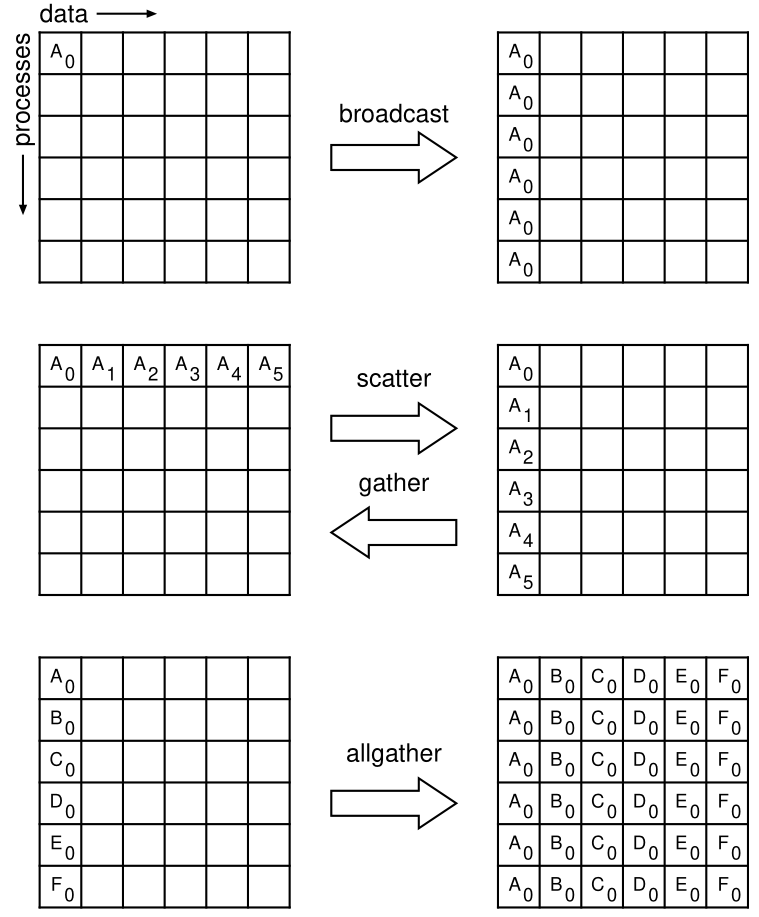
\includegraphics[width = 4.5in]{3_Chapters/2_Chapter_Background/Figs/mpispec_collective.png}
	\caption[Demonstration of collective communications]{
     Demonstration of collective communications taken from \cite{mpi40}.
     Columns specify each process' rank, and rows specify elements in the input vector.
     }
	\label{fig:mpispec_collectives}
\end{figure}

MPI's point-to-point and RMA models specify data transfers between two processes, but often when writing MPI codes, several common patterns arise which require data exchanges among multiple processes at the same time.
These patterns are known as collective communications, and they are common enough that the MPI-forum has standardized several of them.
A few example collectives are outlined in figure \ref{fig:mpispec_collectives}, collectives take a data buffer and transfer the data buffer across all ranks in a communicator.
Collectives can be generalized into two groups, \textit{all-to-one} and \textit{all-to-all} collectives.
All-to-one collectives have a specified root that can act as the main source/destination for all data, for example, \texttt{MPI\_Bcast()} distributes a chunk of data specified by the root to all processes in the communicator.
All-to-all collectives have every process both contribute and receive some set of data within the operations, with, for example, in \texttt{MPI\_Allgather()} each process specifies a segment of data and all the segments are combined into a larger vector (indexed by rank) with a copy of the final result distributed to each process.

The reduction collectives, \texttt{MPI\_Reduce()} and \texttt{MPI\_Allreduce()}, are collectives of particular interest as they are heavily relied upon and can take up large parts of overall application run time.
Their defining characteristic is that accepts an operation which is applied to the data in flight.
\texttt{MPI\_Reduce()} is an all-to-one collective where each process specified a buffer and result is placed at the root, while \texttt{MPI\_Allreduce()} is an all-to-all style collective where each process receives a copy of the final result. 
As an example, if each process had a double and the average across all doubles was necessary for the next step of the computation, each process could call \texttt{MPI\_Allreduce()} with a type \texttt{MPI\_DOUBLE} with the op \texttt{MPI\_SUM} to get the sum of each rank's double, and then divide the result by the communicator size to get the average.

Collective communications are considerably powerful as they can express a lot of data movement in a single operation, and for this reason, they are heavily used in production codes.
But, the inherent downside of collectives is the amount of synchronization they can apply to parallel programs. 
Collectives can be blocking operations, and they require all processes in a communicator to participate in the operation, so they often have the side effect of stalling the entire program waiting for processes to arrive.
Non-blocking collectives do exist, like the point-to-point interface, they return an \texttt{MPI\_Request} object that needs to be progressed with \texttt{MPI\_Test}/\texttt{MPI\_Wait}, but adoption isn't that large and many codes still rely on blocking operations.
The popularity, yet simultaneous optimization challenges, have led to a large body of research on the topic of collective communication. 
There are a plethora of strategies for designing collective algorithms, two of which we rely on for this thesis, including topology-awareness and process arrival pattern awareness.

\subsubsection{Algorithm Structure}\label{sec:CH2-MPI-AlgStructure}
Under the hood, collective algorithms are implemented as a series of point-to-point messages. 
There are different ways to structure the exchanges to implement a specified collective, and different structures have different performance tradeoffs depending on the collective's parameters.
One of the most impactful parameters in communication is the size of the message, and it is best exemplified through Hockney's model \cite{Hockney1994HockenyModel}.
Hockney's model states that the time to send a message of $n$ bytes can be estimated as $T_{msg}=\alpha+n\beta$, where $\alpha$ represents the startup overhead cost (seconds), and $\beta$ is inverse bandwidth (seconds per byte).
What tends to happen in practice is that small messages are bound by $\alpha$, while large messages spend most of their time bandwith bound by $n\beta$.
This principle extends this to collective algorithms, where designs tend to fall into the same two categories, latency bound for small messages and bandwidth bound for large messages, and Thakur et al. provide analysis of most foundational collective algorithms \cite{Thakur2005OptMPICH}.
Latency-bound algorithms try to minimize the number of messages sent as the fewer times we invoke $\alpha$, the faster the algorithm, while large message algorithms will break the data vector into components and issue multiple smaller messages minimizing the total amount of data sent.
When dealing with reduction operations, we can add a $\gamma$ term which represents the time to perform a reduction in seconds per flop, similar to the $\beta$, this scales with $n$.

\begin{figure}
    \centering
    \begin{tikzpicture}[auto]
    
        \def \bkxscale {1.25}
        \def \bkyscale {0.5}
        \begin{scope}[every node/.style={draw, rectangle}, minimum height=0.5cm, minimum width=1.25cm, font=\tiny]
            \foreach \y in {0,1,2,3} \foreach \x in {0,1,2,3} \node at (\x*\bkxscale,\y*\bkyscale) (a\x\y) {$ABCD_{0}$};
            \foreach \y in {10,11,12,13} \foreach \x in {0,1,2,3} \node at (\x*\bkxscale,\y*\bkyscale) (d\x\y) {};
            \foreach \y in {10,11,12,13} \foreach \x in {5,6,7,8} \node at (\x*\bkxscale,\y*\bkyscale) (e\x\y) {};
            \foreach \y\ly in {15/D,16/C,17/B,18/A} \foreach \x\lx in {0cm / 3,1cm / 2,2cm / 1,3cm / 0} \node at (\x*\bkxscale,\y*\bkyscale) (f\x\y) {$\ly_{\lx}$};
            \foreach \y in {15,16,17,18} \foreach \x in {5,6,7,8} \node at (\x*\bkxscale,\y*\bkyscale) (g\x\y) {};
        
            \draw[line width=1pt, double distance=3pt, arrows = {-Latex[length=0pt 3 0]}] (3.5*\bkxscale, 16.5*\bkyscale) -- (4.5*\bkxscale, 16.5*\bkyscale);
            \draw[line width=1pt, double distance=3pt, arrows = {-Latex[length=0pt 3 0]}] (3.5*\bkxscale, 11.5*\bkyscale) -- (4.5*\bkxscale, 11.5*\bkyscale);
            \draw[line width=1pt, double distance=3pt, arrows = {-Latex[length=0pt 3 0]}] (3.5*\bkxscale, 6.5*\bkyscale) -- (4.5*\bkxscale, 6.5*\bkyscale);
            \draw[line width=1pt, double distance=3pt, arrows = {-Latex[length=0pt 3 0]}] (4.5*\bkxscale, 14.5*\bkyscale) -- (3.5*\bkxscale, 13.5*\bkyscale);
            \draw[line width=1pt, double distance=3pt, arrows = {-Latex[length=0pt 3 0]}] (4.5*\bkxscale, 9.5*\bkyscale) -- (3.5*\bkxscale, 8.5*\bkyscale);
            \draw[line width=1pt, double distance=3pt, arrows = {-Latex[length=0pt 3 0]}] (4.5*\bkxscale, 4.5*\bkyscale) -- (3.5*\bkxscale, 3.5*\bkyscale);
            
            \node at (5*\bkxscale, 17*\bkyscale) (comebacktome) {$AB_0$};
            \node at (6*\bkxscale, 16*\bkyscale) (comebacktome) {$BC_1$};
            \node at (7*\bkxscale, 15*\bkyscale) (comebacktome) {$CD_2$};
            \node at (8*\bkxscale, 18*\bkyscale) (comebacktome) {$AD_3$};
            
            \node at (0*\bkxscale, 12*\bkyscale) (comebacktome) {$AB_0$};
            \node at (1*\bkxscale, 11*\bkyscale) (comebacktome) {$BC_1$};
            \node at (2*\bkxscale, 10*\bkyscale) (comebacktome) {$CD_2$};
            \node at (3*\bkxscale, 13*\bkyscale) (comebacktome) {$AD_3$};
            \node at (0*\bkxscale, 11*\bkyscale) (comebacktome) {$ABC_0$};
            \node at (1*\bkxscale, 10*\bkyscale) (comebacktome) {$BCD_1$};
            \node at (2*\bkxscale, 13*\bkyscale) (comebacktome) {$ACD_2$};
            \node at (3*\bkxscale, 12*\bkyscale) (comebacktome) {$ABD_3$};
            
            \node at (5*\bkxscale, 12*\bkyscale) (comebacktome) {$AB_0$};
            \node at (6*\bkxscale, 11*\bkyscale) (comebacktome) {$BC_1$};
            \node at (7*\bkxscale, 10*\bkyscale) (comebacktome) {$CD_2$};
            \node at (8*\bkxscale, 13*\bkyscale) (comebacktome) {$AD_3$};
            \node at (5*\bkxscale, 11*\bkyscale) (comebacktome) {$ABC_0$};
            \node at (6*\bkxscale, 10*\bkyscale) (comebacktome) {$BCD_1$};
            \node at (7*\bkxscale, 13*\bkyscale) (comebacktome) {$ACD_2$};
            \node at (8*\bkxscale, 12*\bkyscale) (comebacktome) {$ABD_3$};
            \node at (5*\bkxscale, 10*\bkyscale) (comebacktome) {$ABCD_0$};
            \node at (6*\bkxscale, 13*\bkyscale) (comebacktome) {$ABCD_1$};
            \node at (7*\bkxscale, 12*\bkyscale) (comebacktome) {$ABCD_2$};
            \node at (8*\bkxscale, 11*\bkyscale) (comebacktome) {$ABCD_3$};
            
            \node at (0*\bkxscale, 7*\bkyscale) (comebacktome) {$AB_0$};
            \node at (1*\bkxscale, 6*\bkyscale) (comebacktome) {$BC_1$};
            \node at (2*\bkxscale, 5*\bkyscale) (comebacktome) {$CD_2$};
            \node at (3*\bkxscale, 8*\bkyscale) (comebacktome) {$AD_3$};
            \node at (0*\bkxscale, 6*\bkyscale) (comebacktome) {$ABC_0$};
            \node at (1*\bkxscale, 5*\bkyscale) (comebacktome) {$BCD_1$};
            \node at (2*\bkxscale, 8*\bkyscale) (comebacktome) {$ACD_2$};
            \node at (3*\bkxscale, 7*\bkyscale) (comebacktome) {$ABD_3$};
            \node at (0*\bkxscale, 5*\bkyscale) (comebacktome) {$ABCD_0$};
            \node at (1*\bkxscale, 8*\bkyscale) (comebacktome) {$ABCD_1$};
            \node at (2*\bkxscale, 7*\bkyscale) (comebacktome) {$ABCD_2$};
            \node at (3*\bkxscale, 6*\bkyscale) (comebacktome) {$ABCD_3$};
            \node at (0*\bkxscale, 8*\bkyscale) (comebacktome) {$ABCD_0$};
            \node at (1*\bkxscale, 7*\bkyscale) (comebacktome) {$ABCD_1$};
            \node at (2*\bkxscale, 6*\bkyscale) (comebacktome) {$ABCD_2$};
            \node at (3*\bkxscale, 5*\bkyscale) (comebacktome) {$ABCD_3$};
            
            \node at (5*\bkxscale, 7*\bkyscale) (comebacktome) {$ABCD_0$};
            \node at (6*\bkxscale, 6*\bkyscale) (comebacktome) {$ABCD_1$};
            \node at (7*\bkxscale, 5*\bkyscale) (comebacktome) {$ABCD_2$};
            \node at (8*\bkxscale, 8*\bkyscale) (comebacktome) {$ABCD_3$};
            \node at (5*\bkxscale, 6*\bkyscale) (comebacktome) {$ABC_0$};
            \node at (6*\bkxscale, 5*\bkyscale) (comebacktome) {$BCD_1$};
            \node at (7*\bkxscale, 8*\bkyscale) (comebacktome) {$ACD_2$};
            \node at (8*\bkxscale, 7*\bkyscale) (comebacktome) {$ABD_3$};
            \node at (5*\bkxscale, 5*\bkyscale) (comebacktome) {$ABCD_0$};
            \node at (6*\bkxscale, 8*\bkyscale) (comebacktome) {$ABCD_1$};
            \node at (7*\bkxscale, 7*\bkyscale) (comebacktome) {$ABCD_2$};
            \node at (8*\bkxscale, 6*\bkyscale) (comebacktome) {$ABCD_3$};
            \node at (5*\bkxscale, 8*\bkyscale) (comebacktome) {$ABCD_0$};
            \node at (6*\bkxscale, 7*\bkyscale) (comebacktome) {$ABCD_1$};
            \node at (7*\bkxscale, 6*\bkyscale) (comebacktome) {$ABCD_2$};
            \node at (8*\bkxscale, 5*\bkyscale) (comebacktome) {$ABCD_3$};
            
        \end{scope}
        
    \end{tikzpicture}
    \caption[Outline of ring allreduce algorithm]{
        Ring allreduce algorithm. Each grid represents a step in the algorithm, where rows are ranks and columns are segments of the data vector.
    }
    \label{fig:ring-allreduce-grid} 
\end{figure}
Figure \ref{fig:ring-allreduce-grid} outlines a four-rank ring-allreduce.
The ring algorithm is often used for large message allreduce because its bandwidth-based performance scales linearly.
During each step of the algorithm, each rank $r$ sends a message to rank $r+1$ and receives a message from rank $r-1$, this is where the ring algorithm gets its name from.
For a ring of $p$ processes, the first $p-1$ steps consist of a data exchange and reduction operation, where each chunk of data consists of $n/p$ Bytes of data. 
At the midway point (the fourth grid in figure \ref{fig:ring-allreduce-grid}), each rank will hold $1/n$ of the fully reduced vector, this data distribution can be considered as a reduce-scatter.
The algorithm finishes with another $p-1$ exchanges of size $n/p$, this time without the reduce, which acts as an allgather distributing the final result.
In total, $2(p-1)$ messages of size $n/p$ are sent, with half of them requiring a reduction, this can give us a total collective time of $T_{ring} = 2(p-1)\alpha + 2((p-1)/p)n\beta + ((p-1)/p)n\gamma$.
The ring algorithm can be generalized to a reduce-scatter followed by an allgather and maintains the $29(p-1)/p)n\beta$ term.
This leads to another popular implementation of allreduce, Rabenseifner's algorithm, which uses a recursive doubling method to implement reduce-scatter allgather \cite{Rabenseifner2004OptOfCollRedOps}.
This change can lower the number of data exchanges to $2\log(p)$ but can require an extra communication stage to balance data if $p$ is not a power of 2.

One-to-all type collective algorithms can often be modelled as trees where vertices are ranks, edges between vertices are messages, and the root of the tree is the root of the collective.
The structure of the tree will have an impact on collective time, for example, a binary tree would theoretically perform better than a linear tree (also known as a chain) due to the logarithmic nature of its height.
Collective algorithms can also leverage message pipelining techniques, where a message is broken into segments and propagated through a tree letting different segments overlap each other.
By default, a chain broadcast would take $T_{chain}=p\alpha+pn\beta$, but with a segment size of $k$ it could be performed in $T_{chain\_pipe}=(n/k+p-1)\alpha+(n+(p-2)k)\beta$.
Pipelining leverages concurrency by propagating data through multiple stages of the tree parallel and shows the most benefit for large message collectives.

While many of these algorithms are foundational to collective research, they tend to make several naive assumptions about the underlying hardware.
Topology-Awareness breaks the assumption that all messages cost the same, as outlined earlier, different interconnects have different performance characteristics, and it has been shown that tailoring the collective structure to the underlying hardware can unlock a lot of performance. 
One other assumption is that all processes arrive at the same time, and process-arrival-pattern-aware collectives break this assumption, they look at how data dependencies within a communication structure can be decoupled to unlock performance.

\subsubsection{Topology Awareness}
Topology awareness, as the name implies, revolves around passing hardware information to the runtime in order to use resources intelligently.
To perform this task, the MPI runtime needs two pieces of information, system hardware information and application communication information.
The hardware information includes the usual suspects like host memory characteristics (NUMA and cache hierarcies), PCIe information on how devices and CPUs are connected, and network characteristics like topology or routing strategy.
This info is relatively easy to collect, there as several libraries for exposing this info to applications, and many MPI implementations already collect this information at runtime.

Acting on topology information is a whole different kind of challenge, these problems involve modelling an application's communication and accelerating it with the hardware info, and many methods have been attempted over the years.
There are ahead of time mapping methods, which involve measuring all communication during a profiling run of an application, using the logs to model a communication pattern, and using the communication pattern to calculate an optimal process to core binding before all future runs of the application. 
Another method of applying topology awareness is virtual topologies, this is a hint applications can pass to the MPI runtime when creating new communicators.
Virtual topologies can include multidimentional cartesian grids or user speicifed graphs, and the MPI implementation can leverage topology information to more optimaly assign ranks in the new communicatior.
Collectives are also a target for topology awareness as the collective itself specifies the expected communication, and the implementation is given free rein to optimize the algorithm however it sees best.

One noteworthy type of topology-aware collective algorithms are hierarchical algorithms, these algorithms break a larger collective into several smaller collectives that run across subsets of the communicator. 
The most basic hierarchy relies on an intranode communicator, where all ranks are on the same node, and an internode communicator, where every rank is on a different node.
Each intranode communicator will select a leader who will be responsible for performing communications across nodes.
In order to perform an allreduce, a typical algorithm could be performed in 4 steps, 1) intranode reduce to the leader, 2) internode reduce to some predetermined rank, 3) internode broadcast, and 4) intranode broadcast.
These algorithms rely on topology information to build hierarchies and are structured to minimize the amount of traffic that has to hit the network. 

\subsubsection{Process Arrival Pattern Awareness}
Process-arrival-pattern awareness leverages process skew to mitigate performance loss or improve application performance. 
Most collective algorithms assume that all ranks enter the collective at the same time, but in reality, performance is not deterministic.
Many stochastic factors can affect compute performance, like OS process scheduling, network noise, and opportunistic CPU frequency boosting, and all these factors can add up to add a skew to process arriving at different times \cite{Faraj2008StudyProcArrivalMPIColl}.

\begin{figure}
    \centering
    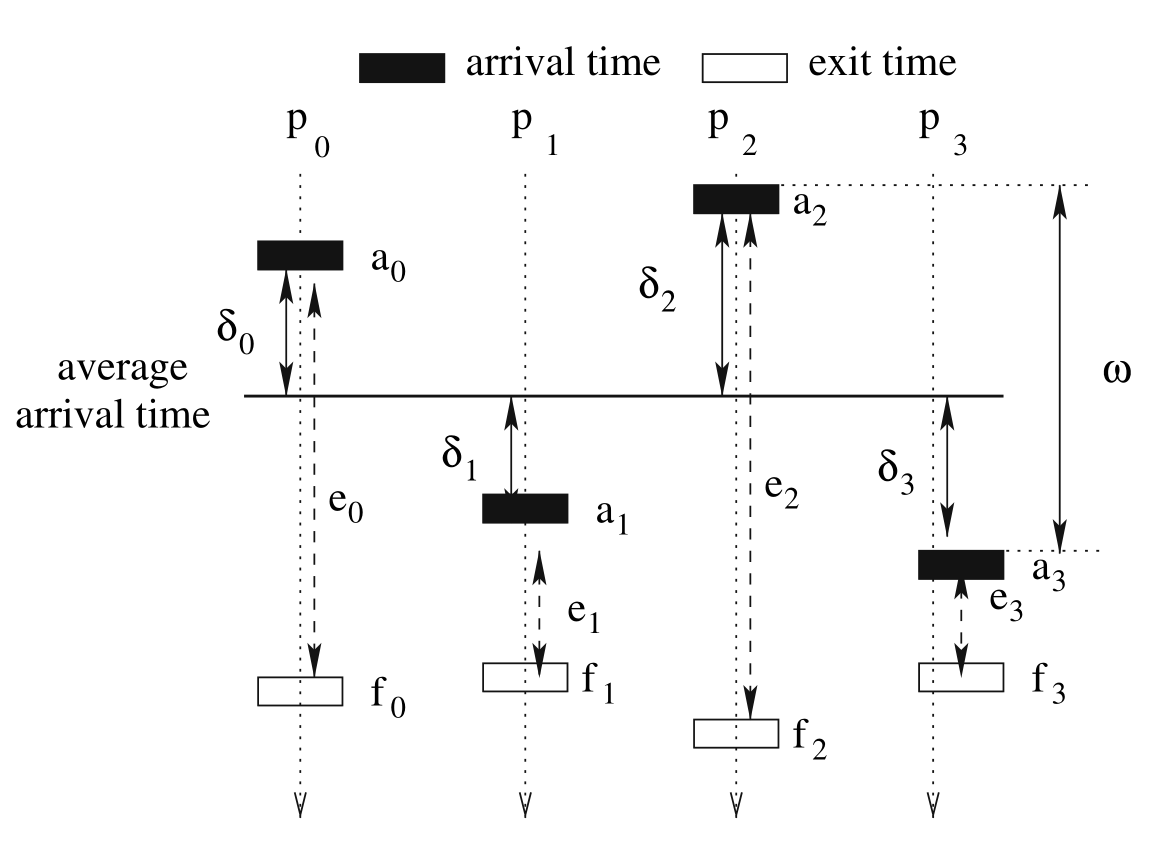
\includegraphics[width=4.5in]{3_Chapters/2_Chapter_Background/Figs/pap_theory.png}
    \caption[Outline of process arrival patterns theory]{
        An outline of process arrival pattern theory for four processes, taken from \cite{Faraj2008StudyProcArrivalMPIColl}.
    }
    \label{fig:pap-theory}
\end{figure}

Faraj et al. \cite{Faraj2008StudyProcArrivalMPIColl} provide a set of formal definitions for modelling process arrivals, a visual interpretation is given in figure \ref{fig:pap-theory}.
For processes $(p_0, p_1,...,p_n)$ participating in a collective operation, each process has an arrival time denoted by $a_i$ and an exit time at $f_n$.
Therefore, each collective call has an arrival patterns $(a_0, a_1, ..., a_n)$ and an exit pattern $(f_0, f_1, ..., f_n)$.
Each rank spends $e_i = f_i - a_i$ time in the collective, where total collective time can be expressed as $e_0 + e_1 + ... + e_n$ and the average collective time is $\bar{e} = (e_0 + e_1 + ... + e_n)/n$, we can use these two terms to evaluate the performance of the overall collective.
In order to quantify the difference between process arrivals, let $\delta_i$ be the absolute time difference between a process's arrival and the average arrival time, i.e. $\delta_i = |\bar{a} - a_i|$. 
We can then define the average arrival imbalance as $\bar{\delta}=(\delta_0 + \delta_i + ... + \delta_n)/n$, and the maximum imbalance time as $\omega = max_i(a_i)-min_i(a_i)$.
When using average/max imbalance in practice, it is often easier to normalize it by the message transmission time.
If the time to send a message of $n$ bytes is $T$, then the \textit{maximum imbalance factor} is of that message is $\omega/T$, and the \textit{average imbalance factor} is $\bar{\delta}/T$.

In order to apply this theory to actual collectives, several problems must be solved.
One of the predominant issues with PAP-Awareness is actually determining the order of process arrival.
Each process needs some level of arrival information to determine the steps it needs to perform within the collective algorithm. 
One strategy for inter-node PAP awareness can include exchanging control messages using MPI point-to-point routines leveraging \texttt{MPI\_ANY\_SOURCE} \cite{Patarasuk2008EffBcastDifProcArr}.
These strategies aren't ideal, as these mechanisms require the active participation of some leader processes.
This is often delegated to the root in one-to-many or many-to-one collectives but doesn't map as easily to many-to-many collectives.
Further, this adds overhead and worsens workload imbalance as one process spends considerably more cycles orchestrating process arrival information.
There is also the issue of processes stalling before the root has arrived, as no work can be done before PAP information is exchanged.
Some proposed work fixes this by delegating PAP management to a background thread \cite{Proficz2018ImprvAllReduceForImbPAP, Proficz2020PAPAwareScatterGather, Proficz2021AllGatherResilientToImbPAP, Faraj2008StudyProcArrivalMPIColl}, but this solution can add more imbalance due to thread scheduling, as well as a burden on application developers to manage resources of background threads.
Other internode solutions rely on non-portable interfaces like RDMA on InfiniBand \cite{Qian2009ProcArrivalSHMA2AIB}.
While this lock the solution to specific hardware, exchanging control messages in a one-sided manner is promising because processes don't synchronize and they can triggers data transfers before other processes have arrived, and they do not rely on a central process managing the entire collective. 

